\section{Implementing the Model}
% \mnote{4.2 provides a "logical view" of the design, ie these are things that have to be supported that
% clearly derive from the quality-centric data model in Chapter 3; one of of thinking about this is that
% this is the "interface" between Chapter 3 and Chapter 4; some of the material from here could be moved
% to 4.3 to make it shorter...}
This section introduces the basic building blocks of our system. It explains how the theoretical concepts
presented in the description of the data model in Chapter~\ref{ch:data_model} can be actually
implemented. It starts describing the basic concepts related to data, namely \textit{tuples} and
\textit{batches}. After that, it covers \textit{operators}, providing a taxonomy and a description of the
most common ones.
It then describes \textit{queries}, showing how they serve as logical containers for operators and can be
partitioned into smaller entities for distribution. Finally, we introduce the \emph{source time window}
that implements the abstract concept of the \emph{source information tuple set}, which associates \sic
values with input tuples.
\vspace{-10pt}
\paragraph*{Tuples.}
\label{sec:tuples}
Tuples are the simplest unit of information processed by a stream processing system.
As described in Section~\ref{sec:definitions}, they comply with a \textit{schema}, stating the number,
the name and the type of their values.
Values represent the \emph{payload} of a tuple (\ie the data processed by operators in a query).
Every tuple also contains a \emph{timestamp}, an indication of their time of creation.
In our system, this is expressed as POSIX time (\ie the number of seconds that have elapsed since
midnight Universal Time Coordinated (UTC) on January 1, 1970).
A timestamp is typically set externally for \emph{base tuples}, or set by the system when creating
\emph{derived tuples}.\\
Tuples are also associated with an individual \sic value, which expresses the quality of the data carried
in the tuple.
In our implementation, this value is associated with the container batch and not attached to each
individual tuple.
This reduces the overhead of transporting a \texttt{double} value (32 bits) with each tuple, exploiting
our assumption that all tuples within a batch have the same \sic value.
\begin{comment}
\lstset{
  basicstyle=\ttfamily,
  columns=fixed,
  showstringspaces=false,
  commentstyle=\color{white}\upshape
}

\lstdefinelanguage{XML}
{
  morestring=[b]",
  %morestring=[s]{>}{<},
  morecomment=[s]{<?}{?>},
  stringstyle=\color{BrickRed},
  identifierstyle=\color{NavyBlue},
  keywordstyle=\color{ForestGreen}, 
  morekeywords={type,name}% list your attributes here
}
\begin{lstlisting}[language=XML,label=lst:tuplexml,caption=XML description of a Tuple]
	<schema name="simpleSchemaONE">
	    <field type="long"   name="ts"  />
	    <field type="double" name="idx" />
	    <field type="double" name="tmp" />  
	</schema>
\end{lstlisting}


As described in Section~\ref{sec:templates}, Tuples are implemented using a template file. One parent
class called ``Tuple'' is provided, containing the basic logic common to all tuples, and every other
tuple class derive from this. In the XML query description, the user specifies a schema and a name for
the tuples that will be used by the query and the system creates a new tuple class, with the name and
fields required. A generic tuple \texttt{.template} file is filled, substituting some placeholders with
the provided data, producing the \texttt{.java} source file of the new tuple class.

Listing~\ref{lst:tuplexml} shows the XML description of a Tuple object with 3 fields: one \texttt{long}
for the timestamp named \textit{ts}, and two \texttt{double}, one with a numerical identifier \textit{idx}
and the other carrying a temperature reading \textit{tmp}. These values will be inserted in the tuple
.template in correspondance with the ``\texttt{\$FIELD}'' placeholder, transforming it into a complete
.java source file. The compiled object will contain 3 public fields with the type and name specified in
 the XML listing.
\end{comment}
\vspace{-10pt}
\paragraph*{Batches.}
\label{sec:batches}
Batches are logical groups of tuples with the same \sic value. Instead of associating an individual
metadata value with each tuple, the system uses batches as containers with a single \sic value, which is
considered valid for all the tuples contained in that batch.\\
Batches are the input and output units of operators. The output of an operator may be composed of
several tuples, which are encapsulated within a batch. The operator calculates a \sic value for all
tuples in the batch based on the \sic values of the input batches and its processing semantics.
The newly produced batch is delivered as input to another operator or is returned as a result to the
user.

Batches are an implementation of the CQL concept of a \textit{relation}, as described in
Section~\ref{sec:cql}.
They represent a finite snapshot of a stream, which allows operators to process a potentially infinite
continuous stream of tuples in consecutive, discrete steps. By using batches, the DISSP system does not
need to use \textit{stream-to-relation} or \textit{relation-to-stream} operators because batches provide
a unified input/output unit for operators. A stream becomes an abstract entity as a potentially infinite set of
batches, while batches serve as the actual units of information in the system.
In our system, batches are simple objects that contain a list of tuples, a \sic value and some additional
metadata. 
% They also contain the logic for converting to and from their network representation.
% --------------------------------   OPERATORS 	--------------------------------	
\paragraph*{Operators.}
\label{sec:operators}
Operators are the basic unit of computation in a stream processing system. They implement a
\textit{function} that transforms one or more input batches to one output batch. A set of operators
linked together in a directed acyclic graph is referred to as a \textit{query}.

Operators can be classified as \textit{blocking} or \textit{non-blocking} based on their behaviour when
handling input data. Many operators can be configured to work in either mode. 
\textit{Blocking operators} need at least one input batch on every input channel before they can
produce an output, while \textit{non-blocking operators} execute every time a new batch of tuples is
delivered on either input. 
% The system implements the logic described in Section~\ref{sec:definitions}.

\begin{figure}
	\centering
	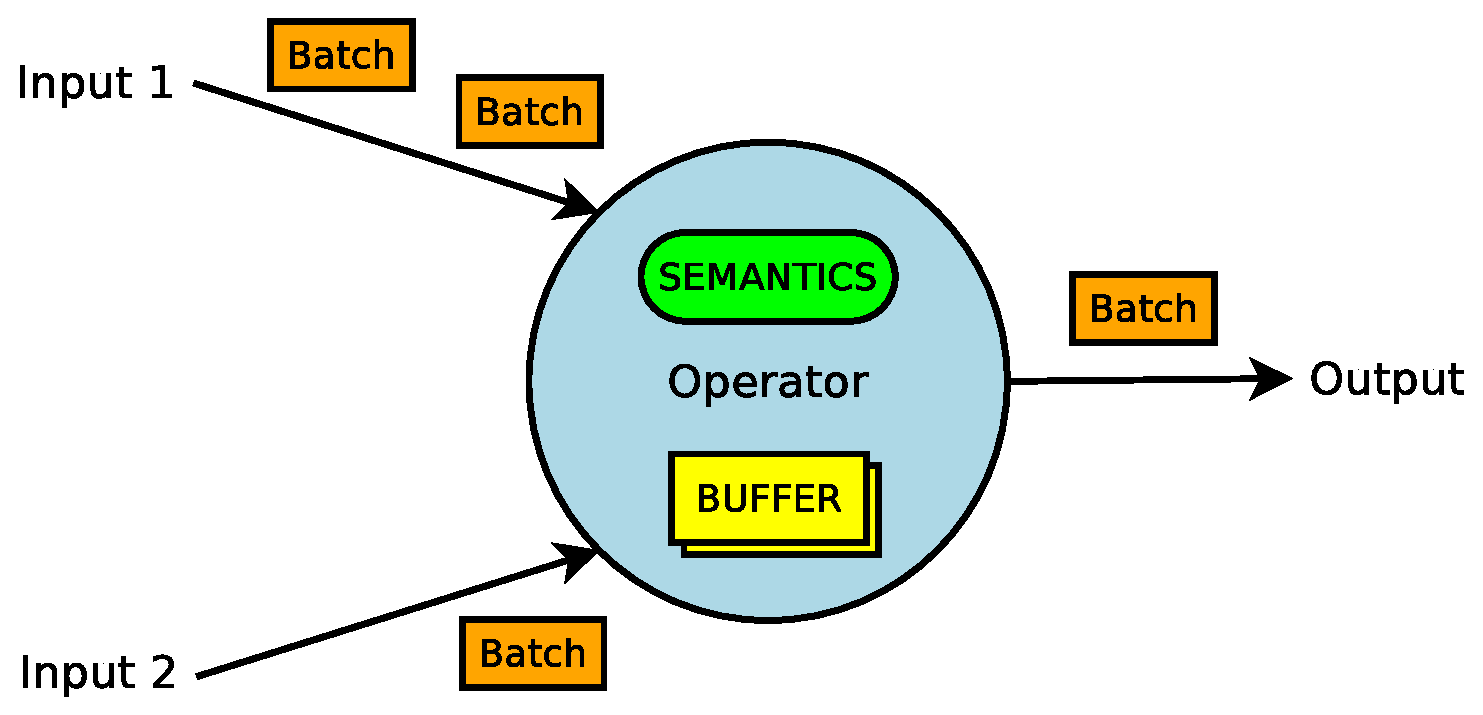
\includegraphics[width=0.6\textwidth]{img/tesi/operator2.eps} 
	\caption{A generic operator with its internal structure shown.}
	\label{fig:op2}
\end{figure}    			

Figure~\ref{fig:op2} shows the internal structure of an operator with its two main components: the
\textit{buffer pool} and the \textit{semantics module}. Every operator is equipped with a pool of
internal buffers, one for each input channel. These are used to stage tuples before they are processed. Every
time an operator triggers for execution, it first moves one or more batches of tuples into the
corresponding buffer within the pool.
A buffer may still contain tuples from the previous execution cycle. In this case,
the new batch is merged with the leftover tuples.

After the input data was staged, the operator executes the logic contained in the \textit{semantics 
module}. This is what characterises an operator by defining its processing logic.
From an implementation point of view, an operator is an abstract class with an unimplemented
\texttt{execute()} function. A concrete operator class has to provide the code for this function. 
Once an operator finished processing, this function returns a batch of tuples that are delivered as its
output.
% From the standpoint of a user, implementing a new custom operator boils down to the definition of
% a new java class, extending either the \textit{BlockingOperator} or the \textit{NonBlockingOperator} class,
% which implements the \texttt{execute()} method. To make this class generic it is then necessary to
% convert it into a \textit{template} file. This is done by replacing some fields with a generic placeholder
% which will then be specified in the XML description of this operator.
\begin{comment}
Listing~\ref{lst:opxml} shows the XML description of an \textit{Average} operator. In the first line the
operator is characterized as being an instance of class ``Average'', described in the correspondent
.template file, and it is given the name of ``MyAvgCpu'. Then there is the declaration of a \textit{next}
operator, this means that this is not a terminal operator and thus its output should be delivered to a
single local operator named ``MyOutput''. Next are 3 parameter definitions, in the form $\langle name,
value \rangle$. The system will look for the ``\$NAME'' placeholder and will replace it with the string
given by ``value''. Once the substitution has taken place, the .template file becomes a complete .java
source file and is then compiled by the \textit{CharSequenceCompiler}.
		 
\lstset{
  basicstyle=\ttfamily,
  columns=fixed,olding,
  showstringspaces=false,
  commentstyle=\color{white}\upshape
}

\lstdefinelanguage{XML}
{
  morestring=[b]",
  %morestring=[s]{>}{<},
  morecomment=[s]{<?}{?>},
  stringstyle=\color{BrickRed},
  identifierstyle=\color{NavyBlue},
  keywordstyle=\color{ForestGreen}, 
  morekeywords={type,name}% list your attributes here
}
\noindent\begin{minipage}{\textwidth}
\begin{lstlisting}[language=XML,label=lst:opxml,caption=XML description of an Average operator]
	<operator name="MyAvgCpu" type="Average">
	    <next name="MyOutput"/>
	    <parameter name="tuple"    value="simpleSchemaONE" />
	    <parameter name="field"    value="cpu"/>
	    <parameter name="groupby"  value="idx"/>
	<operator>
\end{lstlisting}
\end{minipage}

In the next sections there will be an overview of the main classes of operators provided by the DISSP
prototype. \textit{Window Operators} provide transformations over window sizes, holding the input of an
operator until a certain condition is reached. \textit{I/O Operators} are the gateways to the system, in
input they provide the conversion from external to system tuple representation, in output they deliver
the query results to the user. \textit{Network Operators} allow the inter node communication, so that a
query can be partitioned and distributed onto several nodes. Finally there will be a list of the main
\textit{Data Manipulation Operators}, these are the ones actually performing the processing on the data,
and are equivalent to the \textit{relation-to-relation} operators in CQL.

\mnote{Where should I place the operator list? Here seems a bit dispersive}

\subsubsection*{Window Operators}
\label{sec:window-op}
Window Operators provide a way of regrouping tuples, changing the size of their container batches and are
equivalent to the \emph{stream-to-relation} operators in CQL. 
In CQL a stream is a continuous entity and needs to be broken down into a series of relations through a
\emph{stream-to-relation} operator before operators can process it. In our system a stream is a purely 
abstract entity, since batches already are series of tuple snapshots but window operators are still used
to group the input of an operators, so that every new input batch contains tuples with a precise
semantic. The regrouping of tuples can be done according to their \emph{timestamp}, according to the
values of a \emph{field}, or according to their \emph{position} in the stream.

\paragraph{Sliding Windows}


\paragraph{Time Window}
A \emph{Time Window} defines a temporal interval and produces an output batch containing all the tuples
received during the interval. For instance a time window of interval ``1 minute'' outputs a batch of
tuples every minute, containing all tuples received in the previous 60 seconds. The incoming tuples
accumulate in the internal buffers until the current time interval is over, then they are grouped into a
new batch that is sent in output and a new time interval begins. 

\paragraph{Field Window}

\paragraph{Count Window}
A \emph{Count Window} defines a new output batch composed by an exact number of tuples. For instance a
count window of size N always produces batches of N tuples in output. If an input batch contains M
tuples, with M greater than N, it gets broken down into a series of batches of size N, until the
remaining tuples are less than N. These remainder tuples sit in the internal operator buffer until they
are merged with a new incoming batch. When a new batch arrives it is merged with the tuples still present
into the internal buffer from the previous execution and, if their total amount is greater than N, a new
output batch is produced.   

			
	
	
		\subsubsection*{I/O Operators}
		\label{sec:input-output}
			\paragraph{Source Input Device}
			\paragraph{Output Device}
		
		\subsubsection*{Network Operators}
		\label{sec:network-op}	
			\paragraph{Remote Sender}
			\paragraph{Remote Receiver}
		
		\subsubsection*{Data Manipulation Operators}
		\label{sec:data-op}				
			\paragraph{Filter}
			\paragraph{Average}
			\paragraph{Covariance}
			\paragraph{Join}
			\paragraph{TopK}
			\paragraph{Union}
			\paragraph{Min}
			\paragraph{Max}
\end{comment}
% --------------------------------   QUERIES 	--------------------------------		
\paragraph*{Queries.}
\label{sec:queries}

A query logically groups operators that cooperate in the same processing task.
In our design, a query is organised according to the \emph{boxes-and-arrows} model. 
A user submits a query specification containing the list of operators and the connections among them. 
Within a query, operators are organised in a directed acyclic graph. 

A query always starts with one or more \emph{input operators}, which transform the
incoming data streams into the DISSP system format. They thus act as a gateway, allowing external input
generators, such as a sensor network, to connect to the system and make their data available for
processing.\\
In addition, there are a number of \emph{data manipulation operators} that take data items and
process them according to the query semantics. After a final result was obtained, it is delivered to
the user through an \emph{output operator}. 
%The different classes of operators are further described in Section~\ref{sec:operators}.

As described in Section~\ref{sec:fan-in}, the graph of a query have different shapes. Fan-in queries
include a single output operator, while fan-out queries permit for more than one final result and thus
have multiple terminal operators.

\paragraph*{Subqueries.}
Queries may become too computationally expensive to execute completely on a single processing node. 
To avoid overload, the query graph can be split into a number of partitions, which are referred to as
\emph{subqueries}.
The partitioning of a query can follow different strategies, \eg grouping operators according to
equal computational costs or distributing the same subquery for parallel processing. The different query
partitioning schemes are described in Section~\ref{sec:qpart}.

Subqueries are deployed onto several processing nodes. For each query in the system, there is
a \emph{coordinator} that is in charge of the partitioning, deployment and management of the query. It
uses a system of \emph{command messages} to obtain a set of suitable nodes for deployment and to install
the subqueries on the processing nodes. After the query was deployed, data can start flowing
through the input operators and the processing begins.
% --------------------------------   QUERIES 	--------------------------------	
\paragraph*{Source Time Window.}
\label{sec:stw}
Section~\ref{sec:sits} introduced the concept of the \emph{source information tuple set}: the set of
input tuples from which a final result is generated. In the absence of failure, the final \sic value of a
tuple is the sum of the \sic values of all tuples contained in the corresponding source information tuple
set.
According to the model definitions stated in Chapter~\ref{ch:data_model}, every source contributes a
total unnormalised \sic value of $1$ to all result tuples. 
% Every tuple contributing to
% a result passes through an \emph{input operator} and is assigned a \sic value of $1$ divided by the total
% number of participating tuples.

To implement this part of the data model in practice, it would be necessary to know in advance which
tuples will contribute to the creation of a future result. Since the result has not yet been created,
however, it is infeasible to identify the source information tuple set and thus to define it accurately
due to the time delays during query processing caused by processing delays, variable-sized time windows,
etc.
To address this challenge, we consider an approximation: a source information tuple set that includes all
source tuples generated by sources during a predefined time period, referred to as the \emph{source time window (STW)}.

The length of a STW is chosen so that it is always longer than the greatest possible end-to-end query
processing delay.
In this way, the STW contains all tuples that can possibly contribute to the generation of future results.
In practice, a STW may include source tuples that generate multiple different result tuples, or
belong to different source information tuple sets.
Therefore, we apply the same concept of the STW to the result streams as well: the result \sic value of a
query is the aggregate \sic value of all result tuples generated during the same STW.
In order to capture the continuous nature of processing in data streaming, we treat the STW as a
sliding window with a small slide compared to its size.

%%
By using the STW, we no longer require the precise definition of the source information tuple set
$\mathcal{T}^{S}$ and result tuple set $\mathcal{T}^{R}$. Rather, we can use two new sets:
$\mathcal{T}^{S}_{STW}$, which is the set of input tuples belonging to a source time window, and
$\mathcal{T}^{R}_{STW}$, which is the set of output tuples belonging to the corresponding window on
the result streams. 

Using these new tuple sets, the definition of the result \sic value of a query becomes:
\begin{align} 
		\sic_Q = \sum_{t_R \in \mathcal{T}^R_{STW}} t_{R}^{SCR} = \sum_{t_{src} \in \mathcal{T}^{S}_{STW}}
		t_{src}^{SCR},
\end{align}

This definition states that, in the absence of failure, the sum of all \sic values of tuples in a source
time window is equal to the sum of all \sic values of the tuples present in the corresponding window on
the result streams.
% 
% %%
% 
% 
% The \sic value of a derived tuple $t$ processed by operator $o$, \ie $t \in \mathcal{T}_{out}^{o}$, is: 
% % \begin{align} 
% % 	t_{SCR} = \displaystyle\sum_{t \in \mathcal{T}_{in}^{o}}{t_{SCR}} \cdot
% % 	\frac{1}{|\mathcal{T}_{out}^{o}|}
% % \end{align}
% \begin{align} 
% 	t_{SCR} =
% 	\frac{1}{|\mathcal{T}_{out}^{o}|} \cdot \displaystyle\sum_{t \in \mathcal{T}_{in}^{o}}{t_{SCR}} 
% \end{align}
% By using the STW, we no longer require the precise definition of the $\mathcal{T}_{in}^{o}$ and
% $\mathcal{T}_{out}^{o}$ sets. Rather, we can use two new sets for each operator $o$:
% $\mathcal{T}_{in}^{o\prime}$ is formed by the window operator before $o$ and $\mathcal{T}_{out}^{o\prime}$
% depends on the semantics of $o$. Note that $\mathcal{T}_{in}^{o\prime}$ and $\mathcal{T}_{out}^{o\prime}$
% may not contain the correct set of tuples to produce a result tuple. However, we ensure that the
% calculation of the result tuples is correct according to the data model definition of \sic by applying the same STW at the result stream.
% %Section~\ref{sec:eval_stw} will evaluate this approach, showing that the STW correctly captures perfect
% %processing with a negligible error.
